% Set up the document
\documentclass{article}

% Page size
\usepackage[
    letterpaper,]{geometry}

% Lines between paragraphs
\setlength{\parskip}{\baselineskip}
\setlength{\parindent}{0pt}

% Math
\usepackage{amsmath}
\usepackage{amssymb}
\usepackage{mathtools}
\usepackage{physics}

% Shortcut for curly L
\DeclareMathOperator{\Lagr}{\mathcal{L}}

% Links
\usepackage{hyperref}

% Page numbers at top right
\usepackage{fancyhdr}
\pagestyle{fancy}
\fancyhf{}
\fancyhead[R]{\thepage}
\renewcommand\headrulewidth{0pt}

% Graphics
\usepackage{float}
\usepackage{graphicx}
\graphicspath{ {./plots/img/} }

\begin{document}

\textbf{MATH 418 Homework 1} \\
\textbf{Matt Wiens \#301294492} \\
\textbf{2019-09-13}

\textbf{Part 1: Material from MATH 418/718}

1. Determine whether the following equations are linear or nonlinear:

(a) $u \cdot \nabla_{x} u + u = x$

\textbf{Solution}

We can rewrite this equation as $\Lagr(u) = x$ where
$\Lagr(u) = u \cdot \nabla_{x} u + u$. Since
%
\begin{align*}
    \Lagr(c u)
        &= (c u) \cdot \nabla_x (c u) + (c u) \\
        &= c^2 \cdot u \nabla_x u + c u \\
        &= c \left(c \cdot u \nabla_x u + u \right) \\
        &\neq c \left(u \nabla_x u + u \right) \\
        &= c \Lagr(u),
\end{align*}
%
that is, $\Lagr(c u) \neq c \Lagr(u)$, we see that this equation is nonlinear.

\vspace{5mm}
(b) $(1 + t) \partial_{t} u = \partial_{x x} u$

\textbf{Solution}

We can rewrite this equation as $\Lagr(u) = 0$ where
$\Lagr(u) = (1 + t) \partial_{t} u - \partial_{x x} u$. Since
%
\begin{align*}
    \Lagr(u_1 + c u_2)
        &= (1 + t) \partial_{t} (u_1 + c u_2) - \partial_{x x} (u_1 + c u_2) \\
        &= \left( (1 + t) \partial_{t} u_1 - \partial_{x x} u_1 \right)
           + \left( (1 + t) \partial_{t} (c u_2) -  \partial_{x x} (c u_2) \right) \\
        &= \left( (1 + t) \partial_{t} u_1 - \partial_{x x} u_1 \right)
           + c \left( (1 + t) \partial_{t} u_2 -  \partial_{x x} u_2 \right) \\
        &= \Lagr(u_1) + c \Lagr(u_2),
\end{align*}
%
that is, $\Lagr(u_1 + c u_2) = \Lagr(u_1) + c \Lagr(u_2)$, we see that
this equation is linear.

\vspace{5mm}
(c) $\left| \nabla_{x} u \right| = 1$

\textbf{Solution}

We can rewrite this equation as $\Lagr(u) = 1$ where
$\Lagr(u) = \left| \nabla_{x} u \right|$. Using the linearity of
$\nabla$, we have that
%
\begin{align*}
    \Lagr(u_1 + u_2)
        &= \left| \nabla_{x} (u_1 + u_2) \right| \\
        &= \left| \nabla_{x} u_1 + \nabla_{x} u_2 \right| \\
        &\neq \left| \nabla_{x} u_1 \right| + \left| \nabla_{x} u_2 \right| \\
        &= \Lagr(u_1) + \Lagr(u_2);
\end{align*}
%
that is, $\Lagr(u_1 + u_2) \neq \Lagr(u_1) + \Lagr(u_2)$. Hence, this
equation is nonlinear.

\vspace{5mm}
2. Consider the equations
%
\begin{equation}
    \begin{aligned}
        &u_{t} + x u_{x} = u \\
        &u(1, x) = x^2 + 3 x
    \end{aligned}
    \label{eq:p1q2}
\end{equation}
%
(a) Sketch the projected characteristics in the $(t, x)$-plane and label
where the points corresponding to the initial condition are located.

\textbf{Solution}

We can write a system of equations for the projected characteristics as
follows:
%
\begin{equation*}
    \begin{dcases}
        \frac{d t}{d s} = 1 \\
        \frac{d x}{d s} = x \\
        \left( t(0), x(0) \right) = \left( 1, x_0 \right)
    \end{dcases}
\end{equation*}
%
Solving for this system we obtain
%
\begin{align*}
    t(s) &= s + 1 \\
    x(s) &= x_0 \exp(s)
\end{align*}
%
A few of the projected characteristics are plotted below:
%
\begin{figure}[H]
    \centering
    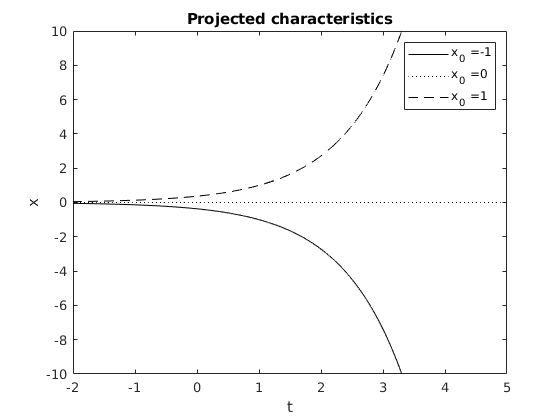
\includegraphics[width=12cm]{p1q2}
\end{figure}

\vspace{5mm}
(b) Solve for $u$ using the method of characteristics.

\textbf{Solution}

Here we have
%
\begin{equation*}
    \frac{d U}{d s} = U
\end{equation*}
%
which has solution
%
\begin{equation*}
    U(s) = (x_0^2 + 3 x_0) \exp(s)
\end{equation*}
%
Now, inverting our equations for $t$ and $s$, we obtain
%
\begin{align*}
    s(t, x) &= t - 1 \\
    x_0(t, x) &= x \exp(1 - t)
\end{align*}
%
and thus we obtain $u(t, x)$ as
%
\begin{align*}
    u(t, x) &= ((x \exp(1 - t))^2 + 3 x \exp(1 - t)) \exp(t - 1) \\
            &= x^2 \exp(1 - t) + 3 x
\end{align*}
%

\vspace{5mm}
(c) Verify that the solution you find indeed satisfies \eqref{eq:p1q2}.

\textbf{Solution}

We calculate (using Maple)
%
\begin{align*}
    u_t &= -x^2 \exp(1 - t) \\
    u_x &= 2 x \exp(1 - t) + 3
\end{align*}
%
and thus
%
\begin{align*}
    &u_t + x u_x \\
    &= \left[
        -x^2 \exp(1 - t)
       \right]
       + x \left[
        2 x \exp(1 - t) + 3
       \right] \\
   &= x^2 \exp(1 - t) + 3 x \\
   &= u
\end{align*}

\vspace{5mm}
\textbf{Part 2: Prerequisite Check}

3. (a) Let $B(\mathbf{0},1)$ be the unit ball in $\mathbb{R}^{3}$ with
   radius $1$. Explicitly compute
%
\begin{align*}
    \iiint_{B(\mathbf{0},1)} &\frac{1}{|\mathbf{x}|} d \mathbf{x} \\
    \iint_{\partial B(\mathbf{0},1)} &\frac{1}{|\mathbf{x}|} d S
\end{align*}

\textbf{Solution}

Here we make use of the radial symmetry of both integrals:
%
\begin{align*}
    \iiint_{B(\mathbf{0},1)} \frac{1}{|\mathbf{x}|} d \mathbf{x}
        &= 4 \pi \int_0^1 r^2 \frac{1}{r} dr \\
        &= 4 \pi \int_0^1 r dr \\
        &= 4 \pi \frac{1}{2} \\
        &= 2 \pi \\
    \\
    \iint_{\partial B(\mathbf{0},1)} \frac{1}{|\mathbf{x}|} d S
        &= \frac{d}{dr} \left(
            \iiint_{B(\mathbf{0},1)} \frac{1}{|\mathbf{x}|} d \mathbf{x}
           \right) \\
        &= \frac{d}{dr} \left(4 \pi \int_0^1 r dr \right) \\
        &= 4 \pi \frac{d}{dr} \left(\int_0^1 r dr \right) \\
        &= 4 \pi
\end{align*}

\vspace{5mm}
For (b) and (c), let $B(\mathbf{0},1)$ be the unit ball in
$\mathbb{R}^{N}$ with radius $1$ and $B^{c}$ its complement, i.e.,
$$B^{c}(\mathbf{0}, 1) = \left\{\mathbf{x} \in \mathbb{R}^{N}: |\mathbf{x}| \geq 1 \right\}$$

(b) For what values of $p > 0$ is the following integral finite?
%
\begin{equation*}
    \int \ldots \int_{B(\mathbf{0}, 1)} \frac{1}{|\mathbf{x}|^{p}} d \mathbf{x}
\end{equation*}

\textbf{Solution}

Let $A$ denote the surface area of the unit sphere in $\mathbb{R}^{N}$.
Then, again exploiting radial symmetry, we have
%
\begin{align*}
    \int \ldots \int_{B(\mathbf{0}, 1)} \frac{1}{|\mathbf{x}|^{p}} d \mathbf{x}
        &= A \int_0^1 r^{N - 1} \frac{1}{r^p} dr \\
        &= A \int_0^1 r^{N - 1 - p} dr \\
        &= A \eval{\qty({\frac{r^{N - p}}{N - p}})}_0^1 \\
\end{align*}
%
which is finite provided $p < N$.

\vspace{5mm}
(c) For what values of $p > 0$ is the following integral finite?
%
\begin{equation*}
    \int \ldots \int_{B^{c}(\mathbf{0}, 1)} \frac{1}{|\mathbf{x}|^{p}} d \mathbf{x}
\end{equation*}

\textbf{Solution}

Again, let $A$ denote the surface area of the unit sphere in
$\mathbb{R}^{N}$. Then we have
%
\begin{align*}
    \int \ldots \int_{B^{c}(\mathbf{0}, 1)} \frac{1}{|\mathbf{x}|^{p}} d \mathbf{x}
        &= A \int_1^\infty r^{N - 1} \frac{1}{r^p} dr \\
        &= A \int_1^\infty r^{N - 1 - p} dr \\
        &= A \eval{\qty({\frac{r^{N - p}}{N - p}})}_1^\infty \\
\end{align*}
%
which is finite provided $p > N$.

\vspace{5mm}
6. Let $f(\mathbf{x}) = |\mathbf{x}|$, where $\mathbf{x} \in \mathbb{R}^{N}$.
Show that $$\nabla f = \frac{\mathbf{x}}{|\mathbf{x}|}$$ More generally,
if $f(\mathbf{x})$ is a radially symmetric function on $\mathbb{R}^{N}$,
that is $$f(\mathbf{x}) = g(|\mathbf{x}|)$$ for some function $g$ on
$\mathbb{R}$, write down an expression for $\nabla f$ in terms of the $g'$.
Use this to find $$\nabla(\sin |\mathbf{x}|)$$

\textbf{Solution}

First we will show that
$f(\mathbf{x}) = |\mathbf{x}| \Rightarrow \nabla f = \frac{\mathbf{x}}{|\mathbf{x}|}$.
For a particular index $x_i$ we have
%
\begin{align*}
    \frac{\partial f}{\partial x_i}
        &= \frac{\partial |\mathbf{x}|}{\partial x_i} \\
        &= \frac{\partial (\sqrt{\sum_{k=1}^n x_k^2})}{\partial x_i} \\
        &= \frac{1}{2 |\mathbf{x}|} \frac{\partial (\sum_{k=1}^n x_k^2)}{\partial x_i} \\
        &= \frac{1}{2 |\mathbf{x}|} \frac{\partial (x_i^2)}{\partial x_i} \\
        &= \frac{x_i}{|\mathbf{x}|}
\end{align*}
%
Hence $\nabla f = \frac{\mathbf{x}}{|\mathbf{x}|}$. Now suppose for some
function $g$, $f(\mathbf{x}) = g(|\mathbf{x}|)$. Then
%
\begin{align*}
    \frac{\partial f}{\partial x_i}
        &= \frac{\partial g(|\mathbf{x}|)}{\partial x_i} \\
        &= g' \frac{\partial |\mathbf{x}|}{\partial x_i} \\
        &= g' \frac{x_i}{|\mathbf{x}|}
\end{align*}
%
Thus $\nabla f = g' \frac{\mathbf{x}}{|\mathbf{x}|}$. Using this to
compute $\nabla(\sin |\mathbf{x}|)$, we have
%
\begin{equation*}
    \nabla(\sin |\mathbf{x}|) = \cos(x) \frac{\mathbf{x}}{|\mathbf{x}|}
\end{equation*}

\vspace{5mm}
7. Let $\mathbf{x} \in \mathbb{R}^{3}$ and
$$u(\mathbf{x}) = \frac{1}{|\mathbf{x}|^{p}}, \quad p>1$$

Calculate the normal derivative $\nabla u \cdot \mathbf{n}$ on $\partial
B(\mathbf{0}, a)$ with the outer normal to $B(\mathbf{0}, a)$.

\textbf{Solution}

\quad \textbf{!!!!!!NOT FINISHED!!!!!}

\vspace{5mm}
8. Verify the Divergence Theorem in $\mathbb{R}^{3}$ for
$\Omega = B(\mathbf{0}, a)$ and vector field $\mathbf{x}$ .

\textbf{Solution}

\quad \textbf{!!!!!!NOT FINISHED!!!!!}

\vspace{5mm}
13. Prove the following ``product rule'' identities for the gradient,
divergence, and Laplacian:

(a) $\nabla(f g) = f \nabla g + g \nabla f,$ for any
$f, g \in C^{1}\left(\mathbb{R}^{3}\right)$

\textbf{Solution}
%
\begin{align*}
    \nabla (f g)
        &= \left\langle
                \frac{\partial (f g)}{\partial x},
                \frac{\partial (f g)}{\partial y},
                \frac{\partial (f g)}{\partial z}
           \right\rangle \\
        &= \left\langle
                f \frac{\partial g}{\partial x} + g \frac{\partial f}{\partial x},
                f \frac{\partial g}{\partial y} + g \frac{\partial f}{\partial y},
                f \frac{\partial g}{\partial z} + g \frac{\partial f}{\partial z}
           \right\rangle \\
        &= \left\langle
                f \frac{\partial g}{\partial x},
                f \frac{\partial g}{\partial y},
                f \frac{\partial g}{\partial z}
           \right\rangle
           +
           \left\langle
                g \frac{\partial f}{\partial x},
                g \frac{\partial f}{\partial y},
                g \frac{\partial f}{\partial z}
           \right\rangle \\
        &= f \left\langle
                \frac{\partial g}{\partial x},
                \frac{\partial g}{\partial y},
                \frac{\partial g}{\partial z}
           \right\rangle
           +
           g \left\langle
                \frac{\partial f}{\partial x},
                \frac{\partial f}{\partial y},
                \frac{\partial f}{\partial z}
           \right\rangle \\
        &= f \nabla g + g \nabla f
\end{align*}

\vspace{5mm}
(b) $\operatorname{div}(f \mathbf{u}) = \mathbf{f} \operatorname{div} \mathbf{u} + \mathbf{u} \cdot \nabla \mathbf{f}$
for any function $f \in C^{1}\left(\mathbb{R}^{3}\right)$ and vector field
$u \in C^{1}\left(\mathbb{R}^{3}, \mathbb{R}^{3}\right)$

\textbf{Solution}

Note: I find the inconsistent(?) use of boldface in the question
confusing, so I'm not going to bold anything in my solution.
%
\begin{align*}
    \operatorname{div}(f u)
        &= \frac{\partial (f u_1)}{\partial x}
           + \frac{\partial (f u_2)}{\partial y}
           + \frac{\partial (f u_3)}{\partial z}
           \\
        &= f \frac{\partial u_1}{\partial x} + u_1 \frac{\partial f}{\partial x}
           + f \frac{\partial u_2}{\partial y} + u_2 \frac{\partial f}{\partial y}
           + f \frac{\partial u_3}{\partial z} + u_3 \frac{\partial f}{\partial z}
           \\
        &= f \left(
            \frac{\partial u_1}{\partial x}
            + \frac{\partial u_2}{\partial y}
            + \frac{\partial u_3}{\partial z}
           \right) +
           u \cdot \left\langle
                \frac{\partial f}{\partial x},
                \frac{\partial f}{\partial y},
                \frac{\partial f}{\partial z}
           \right\rangle \\
        &= f \operatorname{div} u + u \cdot \nabla f
\end{align*}

\end{document}
